\section{Stability Analysis}

\subsection{Introduction}
\par In this section we will lay out a framework for analysing the stability of a numerical method.\\
To begin, we will introduce the concept of the stability function.\\
We will show how it can be used to define a stability region.\\
We will explore the stability region as the set of values for which a numerical method is stable.\\
Finally, we will extend this framework to view the stability of a numerical method in the context of complex time steps.\\

\subsection{Numerical Method: Forward Euler}

\par Let's consider a simple numerical method applied to the Exponential Decay Problem.\\
The Forward Euler method is a first-order numerical method for solving ODEs with a given initial condition.\\
Its algorithm can be defined as:
\[ y(t_{j+1}) = y(t_j) + h y'(t_j)\]
Where $h$ is the time step and $y_j$ is the numerical solution at time $t_j$, $j$ steps on from $t_0=0$.\\
This means $t_j = hj$.\\

\par For the Exponential Decay Problem, the Forward Euler method can be written as:
\[ y_{j+1} = y_j + h \lambda y_j \quad \text{where} \quad y_0 = 1\]
This gives us the following algorithm:
\[ y_{j+1} = (1 + h \lambda) y_j\]
This gives an approximation of the exact solution at time $t_j$ as follows:
\[ y_{j} = {(1 + h \lambda)}^j y_0 = {(1 + h \lambda)}^j = y(t_j) = y(hj) \approx e^{\lh j}\]

\par We can see that the Forward Euler method is stable if $|1 + h \lambda| < 1$;\\
both the exact solution and our approximation will decay to zero as $t \rightarrow \infty$.\\
The stability is dependent on the time step $h$ and the value of $\lambda$.\\
We can write this as $s(\lambda, h) = 1 + h \lambda$.\\
By analysing $s$ for different values of $\lambda$ and $h$,\\
we can infer the stability of the Forward Euler method for the Exponential Decay Problem.\\
We call $s$ the \term{stability function} of the Forward Euler method.

\subsection{The Stability Function and corresponding Stability Region}
\par By the same methodology, we can define the stability function for any numerical method by writing the algorithm in the form $y_{j+1} = s(\lambda, h) y_{j}$.\\
$s(\lambda, h)$ is the \term{stability function} of the numerical method with a time step $h$.\\
\textbf{Note:} This is equivalent to $y_{j} = {s(\lambda,h)}^{j} y_0$

\par The \term{stability region} of a numerical method is the set $S = \Big\{ (\lambda, h) \;\Big|\; |s(\lambda, h)| < 1\Big\} \subset \bC$\\
This follows from the definition of stability for our Exponential Decay Problem;\\
a method is stable if the numerical solution decays to zero as $t \rightarrow \infty$.\\
Clearly, $\Lim{j \rightarrow \infty}y_{j} = \Lim{j \rightarrow \infty}{s(\lambda,h)}^{j} y_0 = 0 \iff |s(\lambda, h)| < 1$.
Now, let's explore some examples of stability regions for different numerical methods.

\newpage
\subsubsection{Stability Region for Euler's Forward Method}
\begin{multicols}{2}
Euler's Forward Method has the stability function
\[s(\lambda, h) = 1 + \lh = \sum\limits_{n=0}^{1} \frac{{(\lh)}^n}{n!} = M(y) + \mathcal{O}((\lh)^2)\]
The corresponding stability region is 
\[S = \Big\{ (\lambda, h) \;\Big|\; |1 + \lh| < 1\Big\}\]
We can see this region plotted in red on the right; an open unit circle centred at $-1$.\\

For a given $\lambda \in \bC$, the method is stable for any step-size $h \in \bR$ such that $|1 + \lh| < 1$.\\

\par Expanding $\lambda = a + bi$, we get the restriction
\[|1 + (a + bi)h| < 1 \quad \implies \quad |(1+ah) + (bh)i| < 1\] 
\[\implies \quad a^2h^2 + 2ah + b^2h^2 < 0\]
\[a, b, h \in \bR \implies (a^2 +b^2)h^2 > 0\] 
\[\implies 2ah < 0 \text{ and } ||2ah|| > (a^2 + b^2)h^2\]
This aligns with our intuition for the problem;
\begin{itemize}
	\item[$\cdot$] For the exponential to decay,\\
	      we must have $Re(\lambda) = a < 0$.
	\item[$\cdot$] $h$ must be positive, as it is a time step.
\end{itemize}
\columnbreak{}
\vspace*{\fill}
\begin{center}
\includegraphics[width=0.49\textwidth]{Stability Regions/Graphs/Real 1-Step/Euler's Forward.png}
See Appendix~\ref{appendix:basic} for the graphing code.\\
\end{center}
\vspace*{\fill}
\end{multicols}
Moreover, 
\[0 < (a^2 +b^2)h^2< ||2ah|| \quad\implies\quad 0 < h < \frac{||2a||}{a^2 + b^2} \quad\implies\quad 0 < h < \frac{2 ||Re(\lambda)||}{{|\lambda|}^2}\]
This is also intuitive; if we imagine $\lambda$ growing linearly, $h$ must shrink quadratically so that their product $\lh$ stays inside the stability region.\\
%\textbf{Note to self: This feels similar to the inversion of a point through a circle in $\bC$.}

\subsubsection{Stability Region for Euler's Backward Method}
\begin{multicols}{2}
\vspace*{\fill}
\begin{center}
\includegraphics[width=0.49\textwidth]{Stability Regions/Graphs/Real 1-Step/Euler's Backward.png}
See Appendix~\ref{appendix:basic} for the graphing code.\\
\end{center}
\vspace*{\fill}
\columnbreak{}
Euler's Backward Method can be written as
\[y_{j+1} = y_j + h.y'(t_{j+1})\]
\[\implies y_{j+1} = y_j + h(\lambda y_{j+1}) \implies y_{j+1} = \frac{1}{1 - \lh}y_j\]
Thus, the stability function is
\[s(\lambda, h) = \frac{1}{1 - \lh}\]
The corresponding stability region is
\[S = \Big\{ (\lambda, h) \;\Big|\; \left|\frac{1}{1 - \lh}\right| < 1\Big\}\]
This is plotted in red on the left; the region outside a unit circle centred at $1$.\\
The white region of instability is exactly the stability region for Euler's Forward Method, flipped about Imaginary axis.\\

\par We could run through the same algebraic procedure as before, expanding $\lambda$ and rearranging, and we would find that 
\[h > \frac{2 Re(\lambda)}{{|\lambda|}^2}\]
\end{multicols}
This is a more lax restriction than the $0<h$ that we have already established.\\
In fact, this tells us that any positive $h$ will give a stable solution, regardless of the value of $\lambda$.\\
This is a property called \term{Absolute Stability} or \term{A-Stability}.\\
This is often characterised by a stability region that covers the entire left half-plane, as we see here.\\

\subsubsection{Stability Region for Runge-Kutta 4}
\begin{multicols}{2}
\vspace*{\fill}

Runge-Kutta 4 can be written as
\[y_{j+1} = y_j + \frac{h}{6}(k_1 + 2k_2 + 2k_3 + k_4)\]
Where $\phi(t,y) = y'(t) = \lambda y$
\begin{flalign*}
	k_1 &= \phi(t_j, y_j) \quad &k_2 = \phi(t_j + \frac{h}{2}, y_j + \frac{h}{2}k_1) && \\
	k_3 &= \phi(t_j + \frac{h}{2}, y_j + \frac{h}{2}k_2) \quad &k_4 = \phi(t_j + h, y_j + hk_3) &&
\end{flalign*}
For the Exponential Decay Problem, we get
\[y_{j+1} = (1 + \lh + \frac{{(\lh)}^2}{2} + \frac{{(\lh)}^3}{6} + \frac{{(\lh)}^4}{24})y_j\]
The stability function is
\[s(\lambda, h) = \sum\limits_{n=0}^{4}\frac{{(\lh)}^n}{n!} = M(y) + \mathcal{O}((\lh)^5)\]
The corresponding stability region is
\[S = \Big\{ (\lambda, h) \;\Big|\; \left|\sum\limits_{n=0}^{4}\frac{{(\lh)}^n}{n!}\right| < 1\Big\}\]

\vspace*{\fill}
\columnbreak{}
\begin{center}
\includegraphics[width=0.49\textwidth]{Stability Regions/Graphs/Real 1-Step/Runge-Kutta 4.png}
See Appendix~\ref{appendix:basic} for the graphing code.\\
\end{center}
\end{multicols}

\newpage
\subsection{Interpretation of Stability Regions}

\par The stability region $S = \Big\{ (\lambda, h) \;\Big|\; |s(\lambda, h)| < 1\Big\} \in \bC$ is a set of values for which a numerical method is stable for the Exponential Decay Problem.\\
We always restrict $h \in {\bR}^{+}$, as it is a time step.\\
We have two separate cases for $\lambda$:
\begin{itemize}
	\item[$\cdot$] $\lambda \in {\bR}^{-}$:\;\; $S$ corresponds to $\big\{{s(\lambda, h)}^2 < 1\big\}$. \;\; Of course, $\lambda, h \in \bR \implies S \subset \bR$.
	\item[$\cdot$] $\lambda \in \bC\setminus\bR$ with $Re(\lambda) < 1$:\;\; $S$ corresponds to $\Big\{\big(s(\lambda, h)\big)\big(\,\overline{s(\lambda, h)}\,\big) < 1\Big\}$.
\end{itemize}

\par From here, one can derive bounds on $h$ for a given value of $\lambda$, or vice versa.\\
We did this with Euler's Forward and Backward methods above.\\
The Runge-Kutta 4 method is more complicated, as the two cases of $\lambda$ each give a polynomial of degree 8.\\

\par Below we have graphs for the cases where $\lambda$ is real or complex,\\
the same as we introduced for the Exponential Decay Problem.\\
In black is the exact solution. In colour are the numerical solutions due to the method in question.\\
These $(\lambda, h)$ pairs were found by first picking a value of $\lambda$ and then finding $h$ values which met the stability condition.\\
In green $(\lambda, h) \in S$.\\
In red $(\lambda, h) \notin S$.\\
Appendix~\ref{appendix:exact_vs_methods} has the code for all graphs in this section.\\
\subsubsection{Euler's Forward Method}
\begin{multicols}{2}
	\begin{center}
	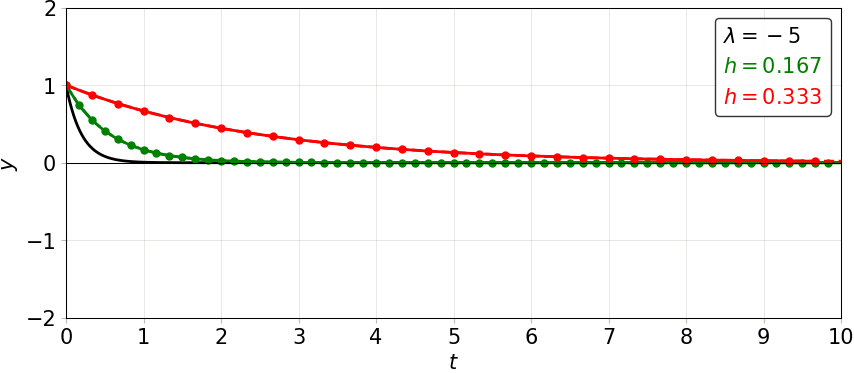
\includegraphics[width=0.49\textwidth]{Exponential Decay/Exact vs Method/Euler's Forward real.png}
        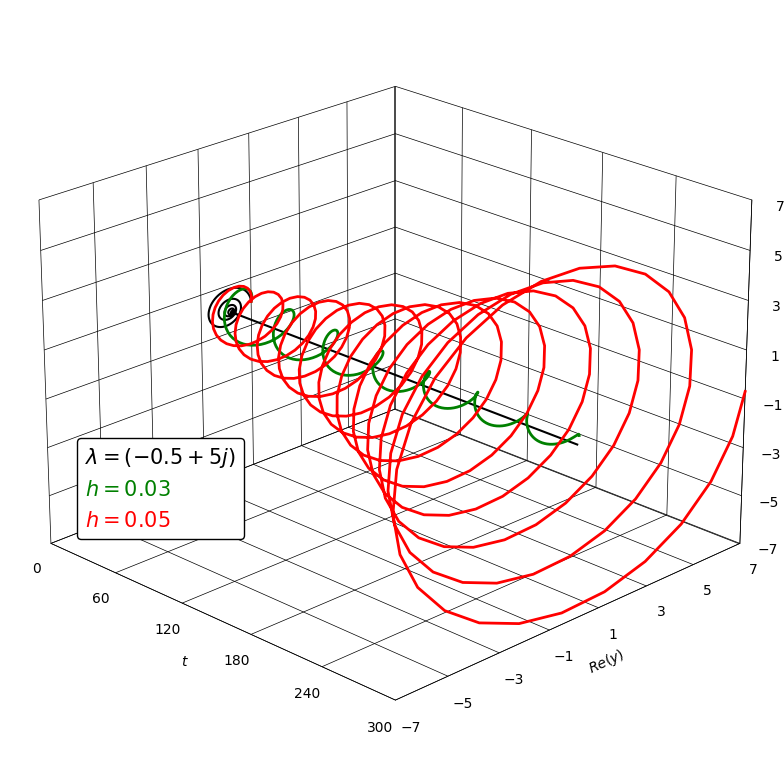
\includegraphics[width=0.49\textwidth]{Exponential Decay/Exact vs Method/Euler's Forward complex.png}
	\end{center}
\columnbreak{}
	\par On the left are the aforementioned graphs for Euler's Forward Method.\\
	
	\par First is the case where $\lambda \in \bR^{-}$.\\
	The exact solution decays quickly in black, very close to $t=0$.
	The numerical solution converges to the exact solution for $h = 1/6$ in green.\\
	For $h = 5/12$, the numerical solution oscillates and diverges in red.\\
	The oscillation is due to the stability function\\
	$s(\lambda, h) = 1 + \lh = 1 + -5\cdot\frac{5}{12} = \frac{-13}{12}$\\
	The $j^{th}$ term of the numerical solution is ${s(\lambda, h)}^j = {\left(\frac{-13}{12}\right)}^j$.\\
	Of course, natural powers of negative numbers oscilate between positive and negative values.\\
	$|\frac{-13}{12}| > 1 \implies$ the numerical solution diverges.\\

	\par Second is the case where $\lambda \in \bC$.\\
	The exact solution decays quickly in black, very close to the $t=0$ plane.\\
	The green, valid $h$ value converges as $t$ increases, but the red, invalid $h$ value diverges.\\
        
        \par While this 3D graph might not be the clearest, it took quite a lot of messing with values of $h$ and $\lambda$ to find one so demonstrative.\\
	The reader is encouraged to play with values for $h$ and $\lambda$ in \\
	Appendix~\ref{appendix:exact_vs_methods} to see for themselves.\\
	This has the added benefit of allowing you to rotate the graph to see the behaviour from different angles.
\end{multicols}
\newpage
\subsubsection{Euler's Backward Method}
\begin{multicols}{2}
	As mentioned before, Euler's Backward Method is A-Stable.\\
	This means that for any $\lambda \in \bC$ with $Re(\lambda) < 1$, the method is stable for any $h \in \bR^{+}$.\\
	As a result, there is no choice of $(\lambda, h)$ that will give us a divergent graph.\\
	For $\lh$ to land in the white disk of instability, either $h$ must be negative or $Re(\lambda) > 1$.\\
	Both of these are nonsensical for our Exponential Decay Problem.\\
	Instead, these graphs show two different stable $h$ values for the same $\lambda$ value.\\
	For $\lambda \in \bR^{-}$ below, the numerical solution converges to the exact solution for both step sizes.\\
	\begin{center}
	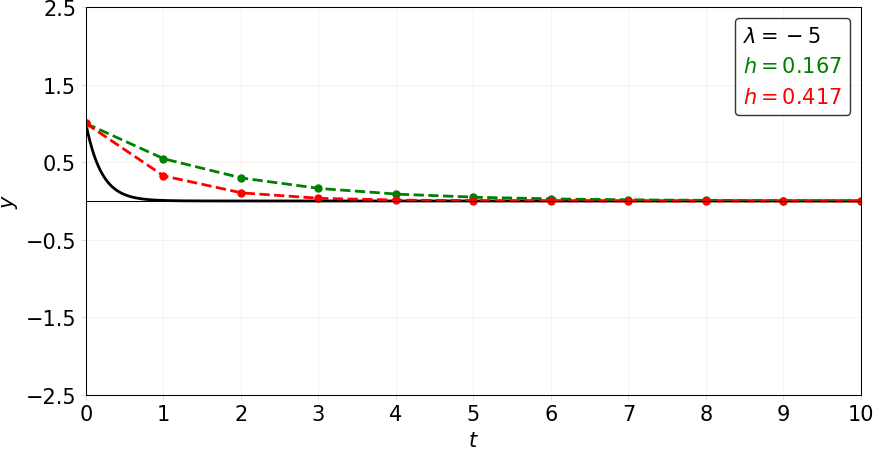
\includegraphics[width=0.49\textwidth]{Exponential Decay/Exact vs Method/Euler's Backward real.png}
	\end{center}
	\columnbreak{}
	\vspace*{-1.5cm}
	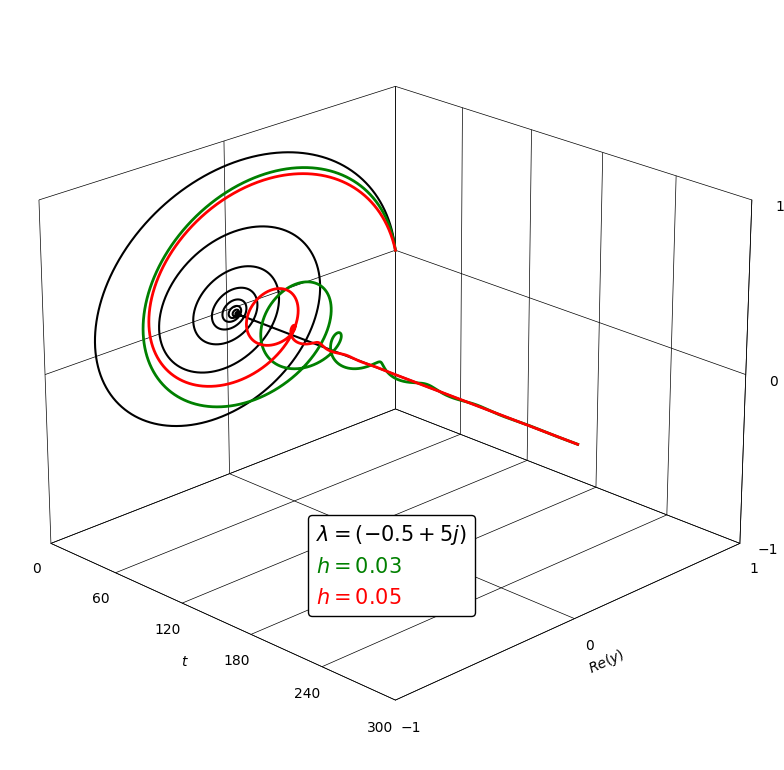
\includegraphics[width=0.49\textwidth]{Exponential Decay/Exact vs Method/Euler's Backward complex.png}
	For $\lambda \in \bC$ above, the method converges to the exact solution for both step sizes.\\
	There is no divergence, as we have already established.\\
	Interestingly, the method converges faster for the larger step size.\\
	The subsequent section on Stability Magnitudes will explain this behaviour.
\end{multicols}
\subsubsection{Runge-Kutta 4}
\begin{multicols}{2}
	The same properties hold true for Runge-Kutta 4, as we demonstrated for Euler's Forward, though we choose different values of $h$ and $\lambda$ for aesthetic clarity.\\
	It was particularly to find a set of values that demonstrated both convergence and divergence, while keeping the exact solution visible.\\
	The lineweight of the unstable $h$ method was decreased to keep everything clear.\\
	\begin{center}
	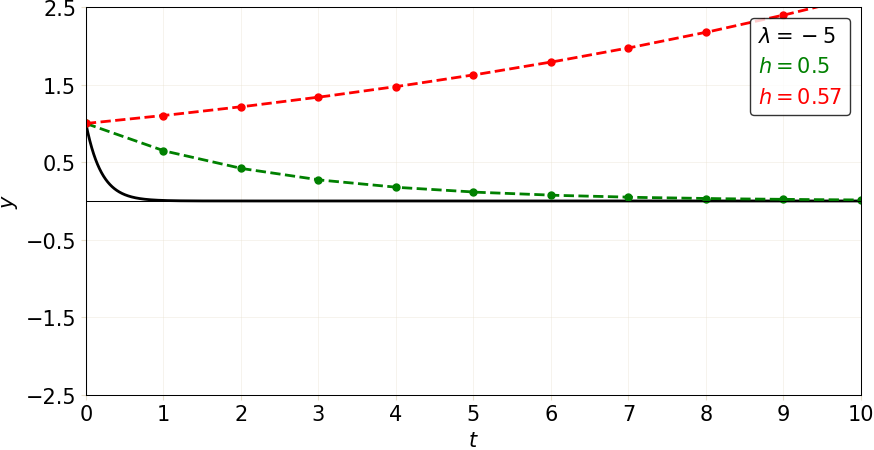
\includegraphics[width=0.49\textwidth]{Exponential Decay/Exact vs Method/Runge-Kutta 4 real.png}
        \end{center}
\columnbreak{}
	\vspace*{-1.5cm}
	\begin{center}
	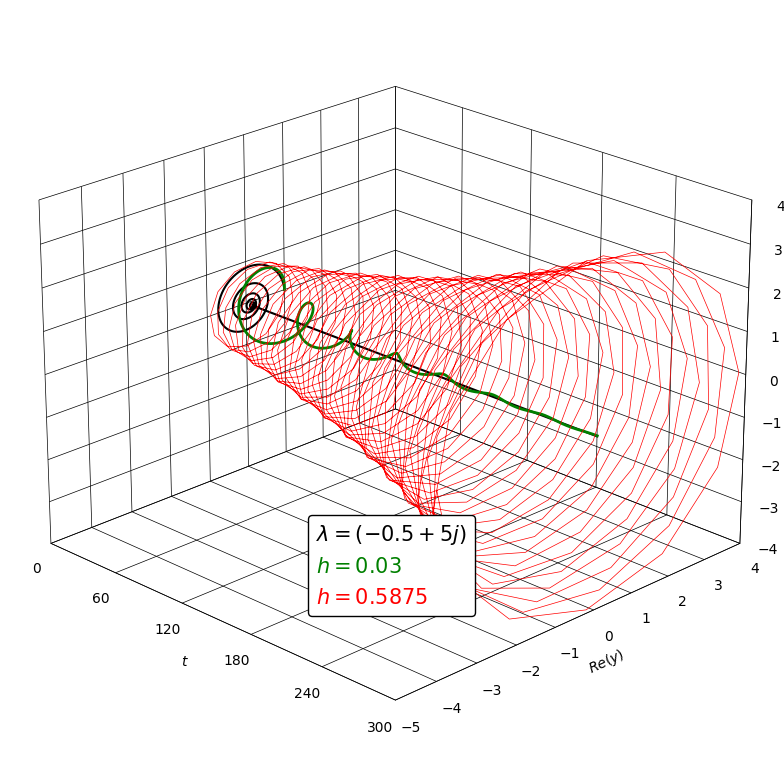
\includegraphics[width=0.49\textwidth]{Exponential Decay/Exact vs Method/Runge-Kutta 4 complex.png}
	\end{center}
\end{multicols}
\newpage
\subsection{Stability Magnitudes}
So far we have been looking at stability regions given by $|s(\lambda, h)| < 1$.\\
While this bound is a sufficient condition for stability, we are not truly utilising the metric.\\
In this section, we'll explore $|s(\lambda, h)|$ in a little more detail.\\
The plots below show the magnitude of the stability function for different values of $\lh$.\\
We have limited these to display only the magnitudes within the region $S$ for clarity; $|s(\lambda, h)| < 1$.\\
The 3D plots show the magnitudes $|s(\lambda, h)|$ above the base plane $S$.\\
The magnitudes have been projected down onto the base plane as colour plots.\\
We show these colour plots separately in the second graphs.\\
While on the first graphs, these colour gradients are continuous, on the second graphs we have discretised them.\\
This is so that for the third graphs we can create a correspondance with the plotted numerical solutions.\\
We'll only present the Exponential Decay graphs for real $\lambda$ here, as the complex $\lambda$ graphs are quite cluttered.\\
Their behavior is the same as for the real $\lambda$ graphs, with tighter, faster decaying spirals as $\lh$ lands in brighter areas of the colour plot.\\
See Appendicies~\ref{appendix:stability_magnitude_3d},~\ref{appendix:stability_magnitude_contour} and~\ref{appendix:stability_magnitude_solutions} for the python used to generate graphs 1, 2 and 3 respectively.\\
\subsubsection{Euler's Forward Method}
\begin{multicols}{2}
	\begin{center}
	\includegraphics[width=0.49\textwidth]{Stability Magnitude/3D/Euler's Forward.png}
	\end{center}
	\columnbreak{}
	\begin{center}
	\includegraphics[width=0.45\textwidth]{Stability Magnitude/Color/Euler's Forward.png}
	\end{center}
\end{multicols}
\begin{multicols}{2}
	\begin{center}
		\includegraphics[width=0.49\textwidth]{Stability Magnitude/Exponential Decay/Euler's Forward.png}
	\end{center}
	\columnbreak{}
	We can see smaller magnitudes correspond to a tighter fit to the exact solution.\\
	This aligns with our intuition; for a derivative,\\
	we allow $h \rightarrow 0$ to obtain the exact solution.\\
	Recall, in a computational context, we're looking for the largest $h$ that will give us a stable solution, that has an error within our tolerance.\\
	Between each point on the graph, $\frac{1}{h}$ calculations are done to find the next point.\\
	For larger $h$, the method is less accurate, but faster.\\
\end{multicols}

\newpage
\subsubsection{Euler's Backward Method}
\begin{multicols}{2}
	\begin{center}
	\includegraphics[width=0.49\textwidth]{Stability Magnitude/3D/Euler's Backward.png}
	\end{center}
	\columnbreak{}
	\begin{center}
	\includegraphics[width=0.45\textwidth]{Stability Magnitude/Color/Euler's Backward.png}
	\end{center}
\end{multicols}
\begin{multicols}{2}
	\begin{center}
		\includegraphics[width=0.49\textwidth]{Stability Magnitude/Exponential Decay/Euler's Backward.png}
	\end{center}
	\columnbreak{}
	As we have already established, Euler's Backward Method is A-Stable.\\
	Any choice of $h \in \bR^{+}$ will give a stable solution for any $\lambda \in \bC$ with $Re(\lambda) < 1$.\\
	It is impossible to pick such $(\lambda, h)$ values that will give $\lambda h$ in the white circle.\\
	By nature of the stability function $s(\lambda, h) = \frac{1}{1 - \lh}$, larger values of $h$ will give a smaller magnitudes; a tighter fit to the exact solution.\\
	This indicates why implicit methods like Euler's Backward are often used for stiff problems; they can be more accurate for larger time steps.\\
\end{multicols}

\subsubsection{Runge-Kutta 4}
\begin{multicols}{2}
	\begin{center}
	\includegraphics[width=0.49\textwidth]{Stability Magnitude/3D/Runge-Kutta 4.png}
	\end{center}
	\columnbreak{}
	\begin{center}
	\includegraphics[width=0.45\textwidth]{Stability Magnitude/Color/Runge-Kutta 4.png}
	\end{center}
\end{multicols}
\begin{multicols}{2}
	\begin{center}
		\includegraphics[width=0.49\textwidth]{Stability Magnitude/Exponential Decay/Runge-Kutta 4.png}
	\end{center}
	\columnbreak{}
	The same general observations as Euler's Forward Method hold true for Runge-Kutta 4.\\
	The values of $h$ here were calculated numerically, rather than algebraically.\\
	The code for calculating these values can be found at Appendix~\ref{appendix:rk4_h}.\\
\end{multicols}
